\documentclass[12pt,a4paper]{article}
\usepackage[a4paper,margin=24mm,headheight=16pt]{geometry}
\usepackage[T1]{fontenc}
\usepackage[utf8]{inputenc}
\usepackage{lmodern}
\usepackage{microtype}
\usepackage{xcolor}
\usepackage{amsmath,amssymb,mathtools}
\usepackage{booktabs,longtable,array,tabularx}
\usepackage{enumitem}
\usepackage{fancyhdr}
\usepackage{hyperref}
\usepackage{tikz}
\usetikzlibrary{arrows.meta,positioning,shapes.geometric,shapes.misc,fit,calc,decorations.pathreplacing,patterns}
\usepackage{pgfplots}
\pgfplotsset{compat=1.18}
\usepackage[most]{tcolorbox}
\usepackage{listings}
\definecolor{navy}{HTML}{183153}
\definecolor{teal}{HTML}{137C8B}
\definecolor{pale}{HTML}{EEF5F7}
\definecolor{orange}{HTML}{C56A20}
\definecolor{rednote}{HTML}{A83232}
\definecolor{greenformula}{HTML}{237A57}
\hypersetup{colorlinks=true,linkcolor=navy,urlcolor=teal,citecolor=teal,pdftitle={Study Notes},pdfauthor={Compiled from Notion study notes}}
\pagestyle{fancy}\fancyhf{}\lhead{\small IIT Madras BS -- Study Notes}\rhead{\small\nouppercase{\leftmark}}\cfoot{\thepage}
\setlength{\parindent}{0pt}\setlength{\parskip}{7pt}\linespread{1.08}
\setlist[itemize]{leftmargin=1.5em,itemsep=4pt,topsep=5pt}
\setlist[enumerate]{leftmargin=1.8em,itemsep=4pt,topsep=5pt}
\newtcolorbox{conceptbox}{colback=pale,colframe=teal!70!black,title=Concept,breakable,fonttitle=\bfseries}
\newtcolorbox{formulaBox}{colback=greenformula!5,colframe=greenformula,title=Core formula,breakable,fonttitle=\bfseries}
\newtcolorbox{exampleBox}{colback=orange!6,colframe=orange,title=Worked example,breakable,fonttitle=\bfseries}
\newtcolorbox{warningBox}{colback=rednote!5,colframe=rednote,title=Common trap,breakable,fonttitle=\bfseries}
\lstset{basicstyle=\ttfamily\small,keywordstyle=\color{navy}\bfseries,commentstyle=\color{teal!70!black},stringstyle=\color{orange!90!black},numbers=left,numberstyle=\tiny\color{gray},numbersep=8pt,frame=single,rulecolor=\color{black!20},breaklines=true,showstringspaces=false,tabsize=4}
\newcommand{\topicflow}[1]{\begin{center}\begin{tikzpicture}[node distance=5mm,>=Latex,every node/.style={draw=teal!70!black,rounded corners,fill=pale,align=center,text width=0.79\linewidth,minimum height=7mm,font=\small}, every path/.style={->,thick,draw=teal}] #1 \end{tikzpicture}\end{center}}
\begin{document}
\begin{titlepage}
\centering\vspace*{20mm}
{\Large\color{teal} IIT MADRAS BS DEGREE PROGRAMME\par}\vspace{12mm}
{\Huge\bfseries\color{navy} Maths for Electronics I\par}\vspace{5mm}
{\Large Calculus, linear systems, series, integration, complex numbers and differential equations\par}\vspace{15mm}
\begin{tcolorbox}[width=0.88\textwidth,colback=pale,colframe=teal]
Expanded learning edition based on the corresponding Notion study guide. This version adds conceptual explanations, worked derivations, guided examples, interpretation of graphs, common-error checks, and practice prompts. It is designed to teach the ideas rather than serve only as a last-minute formula sheet; it is not a verbatim transcript of every lecture.
\end{tcolorbox}
\vfill
\href{https://app.notion.com/p/403a8fc810f681ca96d0e9208f719e6f}{Open original Notion study notes}\par
\vspace{5mm}{\large Compiled 29 October 2026\par}
\end{titlepage}
\tableofcontents\clearpage

\section{Course map and study method}
The Maths for Electronics I course develops one-variable calculus, systems of linear equations, complex numbers, special functions, and ordinary differential equations. Use a cycle of preview, lecture, written derivation, independent practice, error logging, and spaced revision.
\topicflow{\node (a) {Numbers, variables, graphs}; \node (b) [below=of a] {Functions and equations}; \node (c) [below=of b] {Linear systems and matrices}; \node (d) [below=of c] {Sequences, limits, continuity}; \node (e) [below=of d] {Differentiation and applications}; \node (f) [below=of e] {Series and Taylor approximation}; \node (g) [below=of f] {Integration}; \node (h) [below=of g] {Complex numbers and ODEs}; \draw (a)--(b);\draw (b)--(c);\draw (c)--(d);\draw (d)--(e);\draw (e)--(f);\draw (f)--(g);\draw (g)--(h);}
\section{Numbers, variables, functions and equations}
Real numbers include rational and irrational values. A variable may vary; a parameter is fixed within a problem. An expression combines quantities and operations, while an equation asserts equality. A function assigns each allowed input exactly one output.
\begin{itemize}
\item Rational number: $p/q$ for integers $p,q$, with $q\ne0$.
\item For real square roots, the radicand must be non-negative.
\item A real logarithm requires a strictly positive argument.
\item A denominator must not vanish.
\end{itemize}
\subsection{Lines, quadratics and transformations}
A line is $y=mx+c$, where $m=(y_2-y_1)/(x_2-x_1)$ when $x_2\ne x_1$. A quadratic $y=ax^2+bx+c$ ($a\ne0$) has vertex $x=-b/(2a)$ and discriminant $\Delta=b^2-4ac$. Positive, zero, and negative discriminants correspond respectively to two, one repeated, and no distinct real roots.
\begin{itemize}
\item $y=f(x)+k$: vertical shift by $k$.
\item $y=f(x-h)$: horizontal shift right by $h$.
\item $y=af(x)$: vertical scaling by $|a|$, with reflection in the $x$-axis if $a<0$.
\item $y=f(-x)$: reflection in the $y$-axis.
\end{itemize}
\begin{exampleBox}Through $(1,2)$ and $(3,8)$, the slope is $m=(8-2)/(3-1)=3$. Substitution in $y=mx+c$ gives $2=3+c$, so $c=-1$ and $\boxed{y=3x-1}$.
\end{exampleBox}
\begin{center}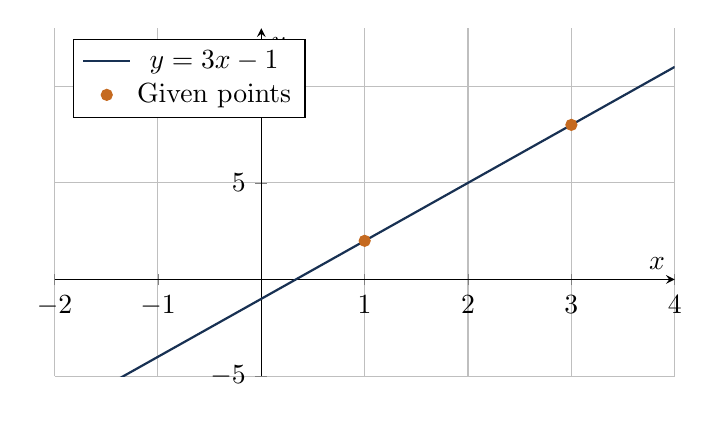
\begin{tikzpicture}\begin{axis}[width=.78\linewidth,height=6cm,axis lines=middle,grid=both,xlabel={$x$},ylabel={$y$},xmin=-2,xmax=4,ymin=-5,ymax=13,legend pos=north west]
\addplot[navy,thick,domain=-2:4,samples=100]{3*x-1};\addlegendentry{$y=3x-1$}
\addplot[orange,only marks,mark=*,mark size=2pt] coordinates {(1,2)(3,8)};\addlegendentry{Given points}
\end{axis}\end{tikzpicture}\end{center}
\subsection{A systematic way to find the domain and range}
The \emph{domain} is the set of inputs for which the rule makes sense. The \emph{range} is the set of outputs the function actually produces. To determine a real-valued domain, begin with all real numbers and remove inputs that violate the formula. For example, for $f(x)=\sqrt{5-2x}$, the radicand must be non-negative: $5-2x\geq0$, hence $x\leq5/2$. For $g(x)=1/(x^2-9)$, require $x^2-9\ne0$, so $x\ne-3,3$.

A useful habit is to write the restriction before simplifying. Cancelling a factor may create an expression that looks defined at a point where the original expression was not defined. The limit of a simplified expression may exist there, but that does not change the original function's domain.

\begin{exampleBox}Find the domain of $h(x)=\sqrt{x+1}/(x-2)$. The square root requires $x+1\geq0$, or $x\geq-1$. The denominator requires $x\ne2$. Therefore the domain is $[-1,2)\cup(2,\infty)$.
\end{exampleBox}

\subsection{Reading a graph before doing algebra}
The graph of a function communicates more than its formula. Check where the graph exists, where it crosses the axes, whether it rises or falls, whether it has turning points, and whether it approaches a value without reaching it. An open circle indicates an excluded point in the graph; a filled point indicates the actual function value. These can differ at the same $x$-coordinate.

\begin{warningBox}Do not infer that a function is one-to-one merely because its formula looks simple. A horizontal line intersecting the graph more than once shows that distinct inputs can share an output. This matters when deciding whether an inverse function exists on the chosen domain.\end{warningBox}

\section{Systems of linear equations and matrices}
A system's solution is a vector satisfying every equation simultaneously. In two dimensions, lines may intersect once (unique solution), be parallel and distinct (no solution), or coincide (infinitely many solutions).
\topicflow{\node (a) {Write equations clearly};\node (b) [below=of a] {Eliminate or substitute};\node (c) [below=of b] {Check the reduced system};\node (d) [below=of c] {Contradiction $0=c$, $c\ne0$: no solution};\node (e) [below=of d] {Consistent: determine pivots and free variables};\node (f) [below=of e] {Pivot for every variable: unique solution};\draw (a)--(b);\draw (b)--(c);\draw (c)--(d);\draw (d)--(e);\draw (e)--(f);}
\subsection{Elimination and matrix form}
For $2x+y=7$ and $x-y=2$, addition gives $3x=9$, so $x=3$. Substitution gives $y=1$.
\[
\begin{bmatrix}2&1\\1&-1\end{bmatrix}\begin{bmatrix}x\\y\end{bmatrix}=\begin{bmatrix}7\\2\end{bmatrix},\qquad
\left[\begin{array}{cc|c}2&1&7\\1&-1&2\end{array}\right].
\]
Elementary row operations preserve the solution set: swap rows, multiply a row by a nonzero constant, or add a multiple of one row to another. A row $[0\;0\mid5]$ encodes the contradiction $0=5$. A variable without a pivot is free.
\subsection{Why row operations are legitimate}
A row operation changes the written system without changing which variable assignments satisfy it. Swapping equations does not change their meaning. Multiplying an equation by a non-zero number produces an equivalent equation. Adding a multiple of one equation to another is also reversible, so it preserves the solution set. These operations are the basis of Gaussian elimination.

\begin{exampleBox}Solve $x+2y=8$ and $3x+2y=12$. Subtract the first equation from the second: $2x=4$, so $x=2$. Substitution into $x+2y=8$ gives $2+2y=8$, hence $y=3$. Check: $2+6=8$ and $6+6=12$. Both original equations are satisfied.
\end{exampleBox}

\subsection{Consistency, pivots, and free variables}
After elimination, a row of the form $0x+0y=5$ is impossible, so the system has no solution. A row $0x+0y=0$ adds no new restriction. If the system is consistent and every unknown has a pivot, the solution is unique. If at least one unknown has no pivot, that variable is free and typically generates infinitely many solutions.

For an $m\times n$ coefficient matrix $A$, the rank counts the number of pivot positions. The rank criterion says that $A\mathbf{x}=\mathbf{b}$ is consistent exactly when $\operatorname{rank}(A)=\operatorname{rank}([A\mid\mathbf{b}])$. If consistent, a unique solution occurs when this common rank equals the number $n$ of unknowns.

\begin{exampleBox}Consider $x+y=4$ and $2x+2y=8$. The second equation is twice the first, so it gives no independent constraint. Let $y=t$; then $x=4-t$. The full solution set is $(x,y)=(4-t,t)$ for real $t$, a line of infinitely many solutions.
\end{exampleBox}

\section{Sequences, boundedness and limits}
A sequence $(a_n)$ is bounded above if $a_n\le M$ for some $M$ and all $n$; bounded below is analogous. It is non-decreasing if $a_{n+1}\ge a_n$ and non-increasing if $a_{n+1}\le a_n$. Convergence to $L$ means that for every $\varepsilon>0$, all sufficiently large $n$ satisfy $|a_n-L|<\varepsilon$.
\begin{itemize}
\item $1/n\to0$.
\item $n$ has no finite real limit.
\item $(-1)^n$ oscillates and does not converge.
\end{itemize}
\begin{formulaBox}Monotone convergence theorem: every monotone increasing sequence bounded above converges; every monotone decreasing sequence bounded below converges.
\end{formulaBox}
\begin{exampleBox}Let $a_1=1$ and $a_{n+1}=(a_n+2)/2$. If $a_n<2$, then $a_{n+1}<2$, and $a_{n+1}-a_n=(2-a_n)/2>0$. The sequence is increasing and bounded above by $2$, hence converges. Its limit $L$ satisfies $L=(L+2)/2$, so $L=2$.
\end{exampleBox}
\begin{center}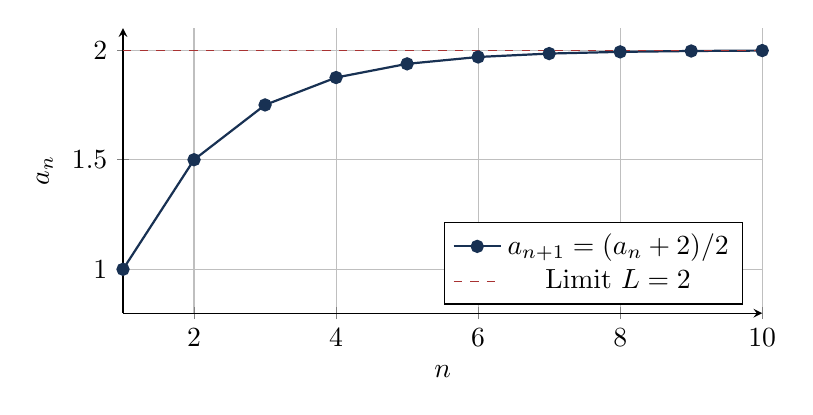
\begin{tikzpicture}\begin{axis}[width=.8\linewidth,height=5.2cm,axis lines=left,grid=major,xlabel={$n$},ylabel={$a_n$},xmin=1,xmax=10,ymin=.8,ymax=2.1,legend pos=south east]
\addplot[navy,thick,mark=*] coordinates {(1,1)(2,1.5)(3,1.75)(4,1.875)(5,1.9375)(6,1.96875)(7,1.984375)(8,1.9921875)(9,1.99609375)(10,1.998046875)};\addlegendentry{$a_{n+1}=(a_n+2)/2$}
\addplot[rednote,dashed,domain=1:10]{2};\addlegendentry{Limit $L=2$}
\end{axis}\end{tikzpicture}\end{center}
\subsection{A reliable proof pattern for sequence limits}
Numerical terms can suggest a limit, but a proof needs a reason that all sufficiently late terms remain close to the proposed value. For recursive sequences, a common strategy is to prove a bound by induction, show monotonicity by examining $a_{n+1}-a_n$, and then apply the monotone convergence theorem. Only after convergence is established should the recurrence be used to solve for the limit.

\begin{exampleBox}Let $b_n=1+1/n$. The first few terms decrease toward $1$. To prove the limit, observe that $|b_n-1|=1/n$. Given any $\varepsilon>0$, choose an integer $N>1/\varepsilon$. For all $n\geq N$, $|b_n-1|=1/n\leq1/N<\varepsilon$. Therefore $b_n\to1$.
\end{exampleBox}

\subsection{Boundedness and monotonicity are separate properties}
A sequence may be bounded without being monotone, as with $a_n=(-1)^n$, which stays between $-1$ and $1$ but oscillates. A sequence may be monotone without being bounded, as with $a_n=n$. The monotone convergence theorem requires both the appropriate monotonicity and a bound in the direction of travel.

\begin{warningBox}Do not confuse a sequence with its series. The sequence $a_n=1/n$ converges to zero, but the series $\sum_{n=1}^{\infty}1/n$ diverges. A sequence asks about individual terms; a series asks about accumulated partial sums.\end{warningBox}

\section{Function limits and continuity}
A limit describes values near a point, not necessarily the value at that point. A two-sided finite limit exists exactly when the left- and right-hand limits exist and agree. Useful techniques include substitution at continuous points, factoring and cancelling on a punctured neighbourhood, rationalisation, standard limits, and separate one-sided analysis for piecewise functions.
\[
\lim_{x\to2}\frac{x^2-4}{x-2}=\lim_{x\to2}(x+2)=4.
\]
A function is continuous at $a$ if $f(a)$ exists, the two-sided limit exists, and the limit equals $f(a)$.
\topicflow{\node (a) {Check that $f(a)$ exists};\node (b) [below=of a,diamond,aspect=2] {Two-sided limit exists?};\node (c) [below left=8mm and 14mm of b] {Not continuous};\node (d) [below right=8mm and 14mm of b,diamond,aspect=2] {Limit equals $f(a)$?};\node (e) [below left=8mm and 12mm of d] {Not continuous};\node (f) [below right=8mm and 12mm of d] {Continuous};\draw (a)--(b);\draw (b)--node[left,draw=none,fill=white]{no}(c);\draw (b)--node[right,draw=none,fill=white]{yes}(d);\draw (d)--node[left,draw=none,fill=white]{no}(e);\draw (d)--node[right,draw=none,fill=white]{yes}(f);}
\subsection{One-sided limits and indeterminate forms}
A two-sided limit at $a$ exists only when the left-hand and right-hand limits agree. For instance, $f(x)=|x|/x$ has left-hand limit $-1$ and right-hand limit $1$ at zero; consequently the two-sided limit does not exist. The fact that $f(0)$ is undefined is not by itself the reason the limit fails—the disagreement between the sides is decisive.

An expression such as $0/0$ is called an indeterminate form: it does not tell us the limit. It may simplify to a finite number, diverge, or behave differently from side to side. For example, $(x^2-1)/(x-1)$ simplifies to $x+1$ for $x\ne1$, giving limit $2$ at $1$. By contrast, $1/x$ has no finite two-sided limit at zero.

\begin{exampleBox}Evaluate $\lim_{x\to0}(\sqrt{x+4}-2)/x$. Direct substitution gives $0/0$. Multiply numerator and denominator by the conjugate:
\[
\frac{\sqrt{x+4}-2}{x}\cdot\frac{\sqrt{x+4}+2}{\sqrt{x+4}+2}
=\frac{1}{\sqrt{x+4}+2}.
\]
Taking $x\to0$ gives $1/4$.
\end{exampleBox}

\subsection{Continuity and types of discontinuity}
Continuity at $a$ requires three things: the value $f(a)$ exists, the two-sided limit exists, and the limit equals the value. A removable discontinuity is a hole that can be filled by redefining one function value. A jump discontinuity occurs when finite one-sided limits differ. An infinite discontinuity occurs when values grow without bound near the point.

\begin{exampleBox}Define $f(x)=(x^2-1)/(x-1)$ for $x\ne1$. Its limit at $1$ is $2$, but the function as written has no value at $1$. If we define $f(1)=2$, the resulting function becomes continuous at $1$.
\end{exampleBox}

\subsection{Limits at infinity for rational functions}
If numerator degree is lower than denominator degree, the limit is $0$. If degrees match, it is the ratio of leading coefficients. If numerator degree is higher, determine the sign and direction carefully; the magnitude typically grows without bound.
\subsection{From average rate to instantaneous rate}
The average rate of change of $f$ between $a$ and $a+h$ is $[f(a+h)-f(a)]/h$. This is the slope of a secant line through two points on the graph. As $h$ approaches zero, the second point moves toward the first. If the slopes approach a finite value, that value is the derivative and the secant approaches the tangent.

\begin{exampleBox}For $f(x)=x^2$, the difference quotient is
\[
\frac{(x+h)^2-x^2}{h}=\frac{2xh+h^2}{h}=2x+h.
\]
Taking $h\to0$ gives $f'(x)=2x$. At $x=3$, the tangent slope is $6$. This tells us that near $x=3$, an increase of approximately $0.01$ in $x$ produces an increase of about $6(0.01)=0.06$ in $f(x)$.
\end{exampleBox}

\subsection{Why the differentiation rules work}
The power rule can be obtained from the difference quotient using the binomial expansion. The product rule follows by adding and subtracting a cross-term in the difference quotient. The chain rule reflects the fact that changes pass through nested functions: the outer rate of change is multiplied by the inner rate of change. These interpretations help determine which rule applies before carrying out algebra.

\begin{exampleBox}Differentiate $y=(x^2+1)(3x-4)$. Using the product rule, $y'=2x(3x-4)+3(x^2+1)=9x^2-8x+3$. Expanding first gives $y=3x^3-4x^2+3x-4$, whose derivative is also $9x^2-8x+3$. The two methods agree.
\end{exampleBox}

\subsection{Implicit differentiation}
Sometimes a relation defines $y$ in terms of $x$ without isolating $y$. Differentiate both sides with respect to $x$, remembering that $y$ depends on $x$. Thus $d(y^2)/dx=2y\,dy/dx$, not simply $2y$.

\begin{exampleBox}For the circle $x^2+y^2=25$, differentiate to obtain $2x+2y\,dy/dx=0$. Rearranging gives $dy/dx=-x/y$ when $y\ne0$. The tangent is horizontal where $x=0$ and vertical where $y=0$, consistent with the geometry of the circle.
\end{exampleBox}

\section{Differentiation and applications}
The derivative is the instantaneous rate of change and tangent slope:
\[
f'(a)=\lim_{h\to0}\frac{f(a+h)-f(a)}{h}.
\]
If $s(t)$ is position, $s'(t)$ is velocity and $s''(t)$ is acceleration. For a time-varying voltage, the derivative quantifies rate of change.
\begin{formulaBox}
\begin{align*}
\text{Power rule: }&\frac{d}{dx}x^n=nx^{n-1},\\
\text{Product: }&(fg)'=f'g+fg',\\
\text{Quotient: }&\left(\frac fg\right)'=\frac{f'g-fg'}{g^2},\quad g\ne0,\\
\text{Chain rule: }&\frac{d}{dx}f(g(x))=f'(g(x))g'(x).
\end{align*}
\end{formulaBox}
Also $(e^x)'=e^x$, $(\ln x)'=1/x$ for $x>0$, $(\sin x)'=\cos x$, and $(\cos x)'=-\sin x$.
\begin{exampleBox}For $y=(3x^2+1)^5$, the chain rule gives
\[
\frac{dy}{dx}=5(3x^2+1)^4(6x)=30x(3x^2+1)^4.
\]
\end{exampleBox}
\begin{center}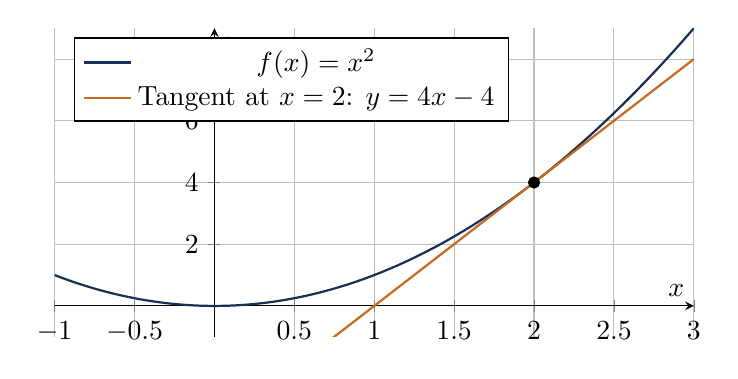
\begin{tikzpicture}\begin{axis}[width=.8\linewidth,height=5.5cm,axis lines=middle,grid=major,xlabel={$x$},ylabel={$y$},xmin=-1,xmax=3,ymin=-1,ymax=9,legend pos=north west]
\addplot[navy,thick,domain=-1:3,samples=100]{x^2};\addlegendentry{$f(x)=x^2$}
\addplot[orange,thick,domain=-1:3]{4*x-4};\addlegendentry{Tangent at $x=2$: $y=4x-4$}
\addplot[only marks,mark=*,mark size=2pt] coordinates {(2,4)};
\end{axis}\end{tikzpicture}\end{center}
\subsection{Second derivatives, concavity, and curve sketching}
The second derivative $f''$ measures how the slope itself changes. If $f''(x)>0$ throughout an interval, the graph is concave up there; if $f''(x)<0$, it is concave down. A point where concavity changes is an inflection point, provided the function is defined there. To sketch a curve, combine intercepts, critical points, intervals of increase/decrease, concavity, and end behaviour rather than relying on a single feature.

\begin{exampleBox}For $f(x)=x^3-3x$, $f'(x)=3x^2-3=3(x-1)(x+1)$. Critical points are $x=-1$ and $x=1$. The derivative is positive for $x<-1$, negative for $-1<x<1$, and positive for $x>1$, so there is a local maximum at $x=-1$ and a local minimum at $x=1$. Since $f''(x)=6x$, concavity changes at $x=0$.
\end{exampleBox}

\section{Mean Value Theorem, monotonicity and approximation}
If $f$ is continuous on $[a,b]$ and differentiable on $(a,b)$, some $c\in(a,b)$ satisfies
\[
f'(c)=\frac{f(b)-f(a)}{b-a}.
\]
If $f'(x)>0$ on an interval then $f$ is strictly increasing; if $f'(x)<0$, it is strictly decreasing. Critical points occur where $f'=0$ or the derivative does not exist while $f$ is defined. A critical point is not automatically an extremum.
\subsection{L'H\^opital's rule}
For suitable differentiable functions in the indeterminate forms $0/0$ or $\infty/\infty$, a ratio limit may be found from the ratio of derivatives if the hypotheses apply. Other forms must be transformed first.
\subsection{Errors and Taylor approximation}
For small increments, $dy=f'(x)\,dx$ and
\[
f(x+\Delta x)\approx f(x)+f'(x)\Delta x.
\]
The Taylor expansion about $a$ is
\[
f(x)\approx f(a)+f'(a)(x-a)+\frac{f''(a)}{2!}(x-a)^2+\cdots.
\]
\subsection{Mean Value Theorem: interpretation and use}
The Mean Value Theorem (MVT) guarantees that a smooth enough function has at least one point where its instantaneous rate equals the average rate across an interval. It is a guarantee of existence; it does not necessarily tell us the point explicitly. The continuity condition on $[a,b]$ and differentiability condition on $(a,b)$ are both essential.

\begin{exampleBox}For $f(x)=x^2$ on $[1,3]$, the average slope is $(9-1)/(3-1)=4$. Since $f'(x)=2x$, the MVT point satisfies $2c=4$, so $c=2$, which lies inside $(1,3)$.
\end{exampleBox}

\subsection{Linearisation and error estimates}
The tangent line at $x=a$ is $L(x)=f(a)+f'(a)(x-a)$. For $x$ close to $a$, $L(x)$ can be easier to calculate than $f(x)$. The approximation improves locally as the increment shrinks, provided the function is differentiable and behaves regularly near the expansion point. A first-order estimate of the absolute output error is approximately $|f'(a)|\,|\Delta x|$.

\begin{exampleBox}Estimate $\sqrt{4.1}$ using $f(x)=\sqrt{x}$ near $a=4$. We have $f(4)=2$ and $f'(x)=1/(2\sqrt{x})$, so $f'(4)=1/4$. Therefore $\sqrt{4.1}\approx2+(1/4)(0.1)=2.025$. The exact value is about $2.0249$, so this is a very accurate local estimate.
\end{exampleBox}

\section{Infinite series and convergence}
A series is interpreted as the limit of partial sums $S_N=\sum_{n=1}^N a_n$. If a series converges, then $a_n\to0$, but the converse is false.
\[
\sum_{n=0}^{\infty} ar^n=\frac{a}{1-r},\quad |r|<1.
\]
The harmonic series $\sum 1/n$ diverges; $\sum 1/n^p$ converges for $p>1$ and diverges for $p\le1$. In the ratio and root tests, $L<1$ establishes absolute convergence and $L>1$ divergence; $L=1$ is inconclusive.
\begin{center}
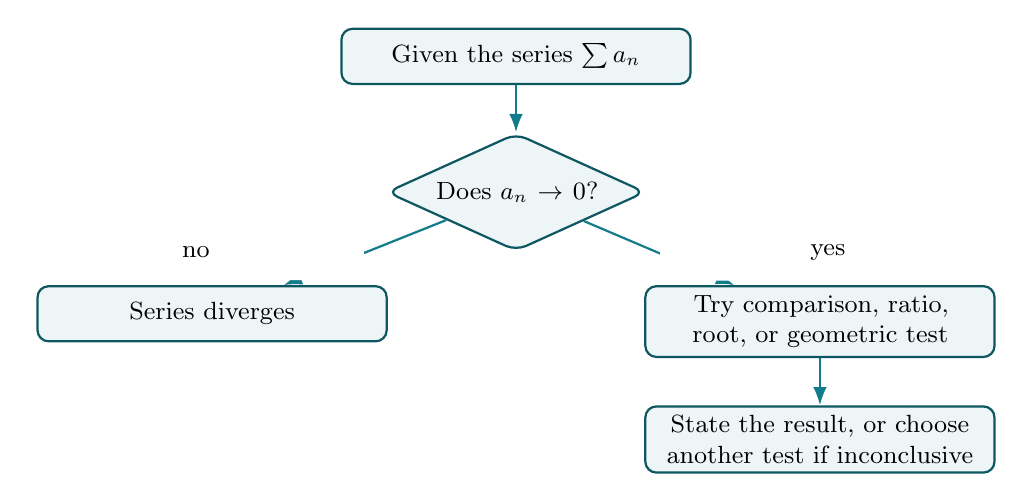
\begin{tikzpicture}[node distance=6mm,>=Latex,
  every node/.style={draw=teal!70!black,rounded corners,fill=pale,align=center,
    text width=4.2cm,minimum height=7mm,font=\small},
  decision/.style={diamond,aspect=2.2,text width=2.5cm,inner sep=1pt},
  every path/.style={->,thick,draw=teal}]
  \node (a) {Given the series $\sum a_n$};
  \node (b) [decision,below=of a] {Does $a_n\to0$?};
  \node (c) [below left=8mm and 8mm of b] {Series diverges};
  \node (d) [below right=8mm and 8mm of b] {Try comparison, ratio, root, or geometric test};
  \node (e) [below=of d] {State the result, or choose another test if inconclusive};
  \draw (a)--(b);
  \draw (b)--node[left,draw=none,fill=white,inner sep=1pt]{no}(c);
  \draw (b)--node[right,draw=none,fill=white,inner sep=1pt]{yes}(d);
  \draw (d)--(e);
\end{tikzpicture}
\end{center}
\subsection{How to choose a convergence test}
Start with the term test: if $a_n$ does not approach zero, the series diverges immediately. If the terms do approach zero, that test gives no conclusion, so inspect the structure.
\begin{itemize}
\item Use the geometric-series formula when consecutive terms have a constant ratio.
\item Use comparison when the terms resemble a known convergent or divergent positive series.
\item Use the ratio test for factorials, products, or expressions containing powers such as $c^n/n!$.
\item Use the root test when the entire term is raised to the $n$th power.
\item Use the $p$-series result for $1/n^p$ and the alternating-series test for suitably decreasing terms with alternating signs.
\end{itemize}

\begin{exampleBox}Determine whether $\sum_{n=1}^{\infty}1/n^2$ converges. Since $p=2>1$, the $p$-series test says it converges. By contrast, $\sum1/n$ has $p=1$ and diverges. The fact that both terms approach zero is not enough to distinguish them; the rate of decay matters.
\end{exampleBox}

\subsection{Partial sums and what convergence means}
A series converges when its partial sums $S_N=a_1+\cdots+a_N$ approach a finite limit. The terms themselves may become small while their accumulated sum continues to grow. For a geometric series, the partial sum is $S_N=a(1-r^{N+1})/(1-r)$ for $r\ne1$; when $|r|<1$, the power $r^{N+1}$ approaches zero and the limiting sum is $a/(1-r)$.

The exponential series is
\[
e^x=\sum_{n=0}^{\infty}\frac{x^n}{n!}=1+x+\frac{x^2}{2!}+\frac{x^3}{3!}+\cdots.
\]
\begin{center}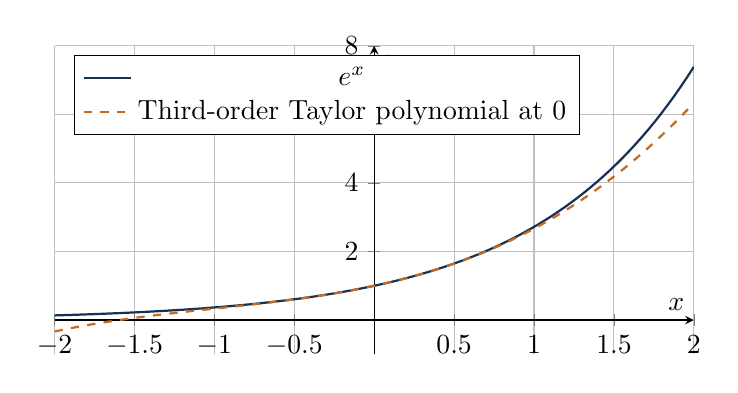
\begin{tikzpicture}\begin{axis}[width=.8\linewidth,height=5.5cm,axis lines=middle,grid=major,xlabel={$x$},ylabel={$y$},xmin=-2,xmax=2,ymin=-1,ymax=8,legend pos=north west]
\addplot[navy,thick,domain=-2:2,samples=100]{exp(x)};\addlegendentry{$e^x$}
\addplot[orange,dashed,thick,domain=-2:2,samples=100]{1+x+x^2/2+x^3/6};\addlegendentry{Third-order Taylor polynomial at $0$}
\end{axis}\end{tikzpicture}\end{center}
\subsection{Alternating series and absolute convergence}
A series $\sum(-1)^{n-1}b_n$ converges by the alternating-series test if $b_n\geq0$, $b_n$ is eventually non-increasing, and $b_n\to0$. Its sum lies between successive partial sums. Absolute convergence means $\sum|a_n|$ converges; absolute convergence guarantees ordinary convergence. Conditional convergence means the original series converges while its absolute-value series diverges.

\begin{exampleBox}The alternating harmonic series $1-1/2+1/3-1/4+\cdots$ converges because $1/n$ decreases to zero. But its absolute-value series is the harmonic series, which diverges. Thus it is conditionally convergent.
\end{exampleBox}

\section{Integration and the Fundamental Theorem}
The definite integral represents signed accumulation. Riemann sums approximate the integral by rectangles of width $\Delta x$:
\[
\sum_{i=1}^{n}f(x_i^*)\Delta x.
\]
If $F'=f$, then $\int_a^b f(x)\,dx=F(b)-F(a)$. Indefinite integrals include an arbitrary constant.
\begin{formulaBox}
\begin{align*}
\int x^n\,dx&=\frac{x^{n+1}}{n+1}+C,\quad n\ne-1,\\
\int \frac{1}{x}\,dx&=\ln|x|+C,\\
\int e^x\,dx&=e^x+C,\\
\int \cos x\,dx&=\sin x+C,\\
\int \sin x\,dx&=-\cos x+C,\\
\int u\,dv&=uv-\int v\,du.
\end{align*}
\end{formulaBox}
\begin{exampleBox}
\[\int_0^2 3x^2\,dx=[x^3]_0^2=8.\]
This is positive geometric area because the integrand is non-negative on the interval.
\end{exampleBox}
\begin{center}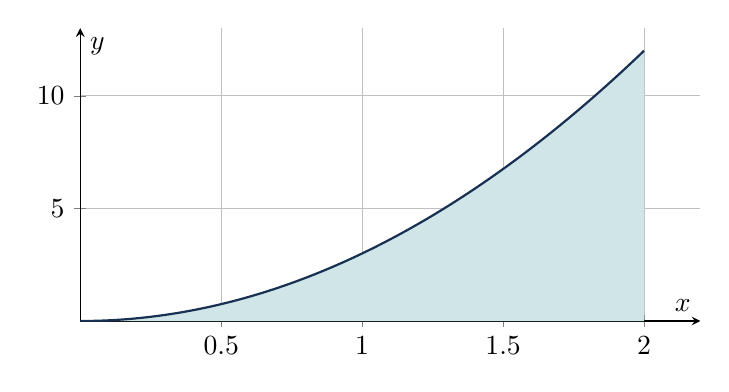
\begin{tikzpicture}\begin{axis}[width=.78\linewidth,height=5.3cm,axis lines=middle,grid=major,xlabel={$x$},ylabel={$y$},xmin=0,xmax=2.2,ymin=0,ymax=13]
\addplot[draw=none,fill=teal!20,domain=0:2] {3*x^2} \closedcycle;
\addplot[navy,thick,domain=0:2,samples=100]{3*x^2};
\end{axis}\end{tikzpicture}\end{center}
\subsection{Integration techniques: choosing a method}
Use direct antiderivatives when the integrand matches a standard rule. Use substitution when the integrand contains a composite expression together with the derivative of its inner function. Use integration by parts for products where differentiating one factor simplifies it. For definite integrals, change the limits when making a substitution or convert back to the original variable before evaluating.

\begin{exampleBox}Evaluate $\int 2x\cos(x^2)\,dx$. Let $u=x^2$, so $du=2x\,dx$. The integral becomes $\int\cos u\,du=\sin u+C=\sin(x^2)+C$.
\end{exampleBox}

\begin{exampleBox}Evaluate $\int xe^x\,dx$. Choose $u=x$ and $dv=e^x\,dx$, so $du=dx$ and $v=e^x$. Then $\int xe^x\,dx=xe^x-\int e^x\,dx=e^x(x-1)+C$.
\end{exampleBox}

\subsection{Signed area versus geometric area}
A definite integral measures signed accumulation: portions below the $x$-axis contribute negatively. Geometric area is non-negative. If a curve crosses the axis, split the interval at the crossings or integrate $|f(x)|$ to calculate total area. In physics, the same distinction appears between displacement (signed integral of velocity) and distance travelled (integral of speed).

\section{Applications of integration}
If $f(x)\ge g(x)$ over $[a,b]$, the area between curves is $A=\int_a^b(f(x)-g(x))\,dx$. If the curves cross, split at intersection points or integrate the absolute difference. Volumes of revolution use disk/washer or shell methods as appropriate. Arc length for a differentiable graph is $\int_a^b\sqrt{1+(y')^2}\,dx$.
\subsection{Area, volume, and arc length in practice}
For area between curves, identify which function is on top on each subinterval. If the top and bottom functions swap order, split the interval at their intersections. For solids of revolution, disks use $V=\pi\int_a^b R(x)^2\,dx$; washers use $V=\pi\int_a^b(R(x)^2-r(x)^2)\,dx$, where $R$ and $r$ are outer and inner radii. Shell methods are useful when cylindrical shells produce a simpler integral.

\begin{exampleBox}The area under $y=x$ from $x=0$ to $x=2$ is $\int_0^2x\,dx=[x^2/2]_0^2=2$. Rotating this region about the $x$-axis gives a cone-like solid with volume $\pi\int_0^2x^2\,dx=8\pi/3$.
\end{exampleBox}

\section{Complex numbers and polar form}
A complex number is $z=a+ib$, where $i^2=-1$. Its conjugate is $\bar z=a-ib$ and modulus $|z|=\sqrt{a^2+b^2}$. For $z\ne0$, $z\bar z=|z|^2$ and
\[
\frac{a+ib}{c+id}=\frac{(a+ib)(c-id)}{c^2+d^2},\quad c+id\ne0.
\]
Polar form is $z=r(\cos\theta+i\sin\theta)=re^{i\theta}$ where $r=|z|$ and $\theta$ is an argument. Multiplication multiplies magnitudes and adds arguments; division divides magnitudes and subtracts arguments.
\begin{center}\begin{tikzpicture}[scale=1.0,>=Latex]\draw[->] (-.3,0)--(4.4,0) node[right] {$\Re$};\draw[->] (0,-.3)--(0,3.2) node[above] {$\Im$};\draw[navy,very thick,->] (0,0)--(3,2.2) node[midway,above left] {$r$};\draw[orange,thick] (1,0) arc (0:36.25:1);\node at (1.25,.42) {$\theta$};\fill (3,2.2) circle (2pt);\node[above right] at (3,2.2) {$a+ib$};\end{tikzpicture}\end{center}
\subsection{Complex-number operations and geometry}
Complex numbers behave like ordered pairs $(a,b)$ with an extra multiplication rule determined by $i^2=-1$. Addition is componentwise: $(a+ib)+(c+id)=(a+c)+i(b+d)$. Multiplication follows distribution and replacement of $i^2$ by $-1$: $(a+ib)(c+id)=(ac-bd)+i(ad+bc)$. The conjugate changes the sign of the imaginary part and is useful for division because $(a+ib)(a-ib)=a^2+b^2$.

\begin{exampleBox}Compute $(2+3i)(1-2i)$. Expanding gives $2-4i+3i-6i^2$. Since $i^2=-1$, this becomes $2-i+6=8-i$.
\end{exampleBox}

In polar form, $z=re^{i\theta}$. Multiplying two non-zero complex numbers multiplies their moduli and adds their arguments; dividing divides moduli and subtracts arguments. De Moivre's formula states $(r(\cos\theta+i\sin\theta))^n=r^n(\cos n\theta+i\sin n\theta)$ for integer $n$, and is particularly useful for powers and roots.

\section{Differential equations and final revision}
A first-order ordinary differential equation relates an unknown function and its derivative. For separable equations, rearrange to $g(y)\,dy=f(x)\,dx$ and integrate both sides, checking the domain and any division by zero. Linear first-order equations have form $y'+p(x)y=q(x)$ and may be solved using the integrating factor $\mu(x)=e^{\int p(x)\,dx}$.
\begin{itemize}
\item Identify domains before manipulating limits or functions.
\item Verify every solution in the original equation when possible.
\item State the hypotheses of convergence and calculus theorems.
\item Track signs, constants of integration, endpoints, and units.
\item Practise proofs and mixed problems without notes.
\end{itemize}
\subsection{Separable equations: a worked solution}
For a separable equation, rearrange the equation so that all terms involving $y$ are on one side and all terms involving $x$ are on the other. Integrate both sides, then solve for $y$ if possible. Be careful: dividing by a function of $y$ can discard constant solutions where that function is zero, so check those separately.

\begin{exampleBox}Solve $dy/dx=2xy$. For $y\ne0$, separate variables: $dy/y=2x\,dx$. Integrating gives $\ln|y|=x^2+C$, so $y=Ce^{x^2}$ after absorbing the sign into the constant. The solution $y=0$ is included when $C=0$.
\end{exampleBox}

\subsection{First-order linear equations}
A linear first-order equation has the form $y'+p(x)y=q(x)$. Its integrating factor is $\mu(x)=e^{\int p(x)\,dx}$. Multiplying through gives $(\mu y)'=\mu q$, so integration yields $\mu y=\int\mu q\,dx+C$ and then $y$ is found by dividing by $\mu$.

\begin{exampleBox}Solve $y'+y=1$. The integrating factor is $e^{\int1\,dx}=e^x$. Thus $(e^xy)'=e^x$, so $e^xy=e^x+C$, and $y=1+Ce^{-x}$. Substitution into the original equation confirms the solution.
\end{exampleBox}

\section{Topic-by-topic self-test}
Try answering each prompt without looking at the preceding section. If you cannot explain the reasoning aloud, revisit the worked example and solve a similar problem with different values.
\begin{enumerate}
\item \textbf{Functions:} Determine the domain of $\sqrt{3-x}/(x+2)$ and explain both restrictions.
\item \textbf{Linear systems:} Explain how a row $[0\;0\mid c]$ with $c\ne0$ proves inconsistency.
\item \textbf{Sequences:} Give one bounded non-monotone sequence and one monotone unbounded sequence.
\item \textbf{Limits:} Evaluate $\lim_{x\to3}(x^2-9)/(x-3)$ and explain why substitution alone is inconclusive.
\item \textbf{Continuity:} State the three conditions required for continuity at a point.
\item \textbf{Derivatives:} Differentiate $(2x+1)^4$ and identify the inner derivative explicitly.
\item \textbf{Applications:} Find the critical points of $x^3-3x$ and classify them using the first derivative.
\item \textbf{Series:} Explain why $a_n\to0$ is necessary but not sufficient for $\sum a_n$ to converge.
\item \textbf{Integration:} Evaluate $\int_0^1 4x^3\,dx$ and distinguish signed area from total geometric area.
\item \textbf{Complex numbers:} Find the modulus and conjugate of $3-4i$.
\item \textbf{ODEs:} Solve $y'=3y$ and verify the solution by differentiation.
\end{enumerate}

\section{Source and scope}
Source: \href{https://app.notion.com/p/403a8fc810f681ca96d0e9208f719e6f}{Maths for Electronics 1 -- Complete Study Notes and Visual Revision Guide}; official course outline: \url{https://study.iitm.ac.in/ae/course_pages/BSMA1101.html}. The LaTeX version typesets the main syllabus notes and diagrams in a self-contained format; use the live course portal for current assessment requirements and instructor-specific notation.
\end{document}
